\subsection{\SubsecCopyTopo} \label{subsec:nest_topo}
%------------------------------------------------------
ネスティング実験では、一般的に、親領域と子領域の間で空間解像度が異なるため地形の解像度も異なる。
子領域の緩和領域(第\ref{subsec:buffer}節を参照)では、大気の変数は親領域の変数へとナッジングされる。
2つの領域間で地形の表現が異なると、親領域で計算されるナッジングのための参照データが存在しないことがある。
その場合は外挿により大気データを見積もることになるが、外挿による見積もりの精度が悪いと不整合が生じる。
%
地形の違いによる不整合を回避するために、
\scalerm では「地形コピー」機能の使用を推奨している。
この機能は、子領域の緩和領域における地形として親領域の地形をコピーする。
この機能を使えば、図\ref{fig_topocopy}に示すように、子領域における緩和領域の地形を
親領域の地形と完全に一致させられる。
さらに、地形の解像度を外側から内側に行くに従って徐々に高めるために、
緩和領域の内側に地形の遷移領域を置く。
地形の遷移領域では、地形は親領域と子領域の地形を重み付けすることで生成される。
地形遷移領域の幅は、デフォルト設定では緩和領域と同じ幅である。
これよりも内側の計算領域では、地形は子領域の地形を与える。
「実験セット一式準備ツール」(第\ref{sec:basic_makeconf}節)を利用する場合には、
地形コピー機能は自動的に適用される。


本節で示す\verb|pp.d0*.conf|ファイルは、サンプル設定ファイル\\
\verb|${Tutorial_dir}/real/sample/USER.online-nesting.sh|を
USER.shに名前を変更して、「実験セット一式準備ツール」を実行することで作成される。
説明を読み進める上で参考にしてもらいたい。
以降は、具体的な設定方法と実行手順を説明する。


\begin{figure}[htb]
\begin{center}
  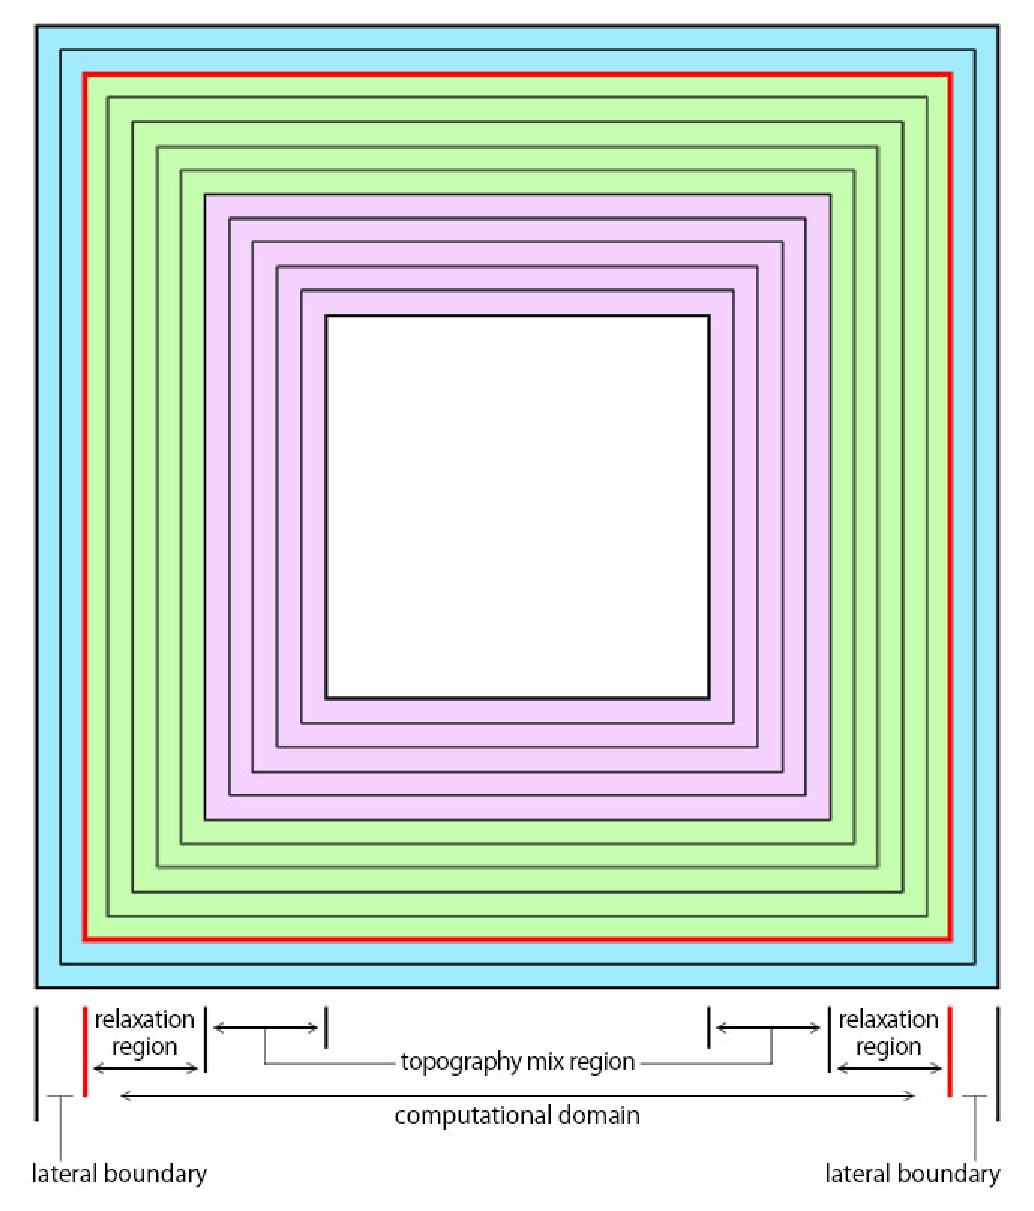
\includegraphics[width=0.4\hsize]{./figure/topo_copy.pdf}\\
  \caption{地形コピー機能を適用したときの地形の水平分布。
水色で塗られた最外にある格子は\texttt{HALO}領域であり、
その格子数は水平移流スキームに依存する。
これらの格子は側面境界である。
赤色の線で囲われた部分は、計算領域である。
緑色や桃色の領域はそれぞれ、緩和領域と地形遷移領域である。
最内の白色の領域では、地形は子領域のもとの地形と同じである。
地形遷移領域では、外側から内側にかけて徐々に親領域の地形データから子領域の地形データへ遷移する。}
  \label{fig_topocopy}
\end{center}
\end{figure}


\subsubsection{地形コピー機能の使い方}

親領域の地形データを\verb|scale-rm_pp|によって作成する際に、
親領域の大きさを子領域に与えるためのカタログファイルを出力させるためには、
下記の設定が\verb|pp.d01.conf|に必要である。\\
\editboxtwo{
\verb|&PARAM_DOMAIN_CATALOGUE|  & \\
\verb| DOMAIN_CATALOGUE_FNAME  = "latlon_domain_catalogue.d01.txt",| & カタログファイルのファイル名\\
\verb| DOMAIN_CATALOGUE_OUTPUT = .true.,| & カタログファイルを出力するかどうか \\
\verb|/|  & \\
}
その他の設定項目は通常通りで良い。

次に、地形コピー機能で親の地形を用いるために、
以下のように子領域に対する\verb|pp.d02.conf|ファイルを編集する。
ここでは、親領域の地形の出力データが\verb|topo_d01.pe***.nc|として保存されていると想定する。

\noindent {\small {\gt
\ovalbox{
\begin{tabularx}{150mm}{lX}
\verb|&PARAM_NEST| & \\
\verb| OFFLINE_PARENT_BASENAME   = "topo_d01", | & 親領域のファイルのベース名 \\
\verb| OFFLINE_PARENT_PRC_NUM_X  = 2,          | & 親領域の\verb|PRC_NUM_X| \\
\verb| OFFLINE_PARENT_PRC_NUM_Y  = 2,          | & 親領域の\verb|PRC_NUM_Y| \\
\verb| LATLON_CATALOGUE_FNAME    = "latlon_domain_catalogue.d01.txt",| & 親領域のカタログファイル  \\
\verb|/| &\\
 & \\
\verb|&PARAM_CNVTOPO|  &\\
\verb|     〜 中略 〜| & \\
\verb| CNVTOPO_copy_parent     = .true.,| & 地形コピー機能を適用するかどうか\\
\verb|/| &\\
 & \\
\verb|&PARAM_COPYTOPO| & \\
\verb| COPYTOPO_IN_BASENAME   = "topo_d01",| & 親領域の地形データファイルのベース名 \\
\verb| COPYTOPO_TRANSITION_DX = -1,        | & x方向の遷移域の幅 \\
\verb| COPYTOPO_TRANSITION_DY = -1,        | & y方向の遷移域の幅 \\
\verb| COPYTOPO_ENTIRE_REGION = .false.,|    & 子領域の全域に親領域の地形をコピーするかどうか\\
\verb| COPYTOPO_LINEAR_H      = .true.,|     & \\
\verb|/| & \\
\end{tabularx}
}}}\\

\noindent
\namelist{PARAM_CNVTOPO}の\nmitem{CNVTOPO_copy_parent}を\verb|.true.|とすれば、
地形のコピー機能が適用される。
\nmitem{COPYTOPO_ENTIRE_REGION}は、子領域の全域に渡って親領域の地形をコピーするかどうかのオプションである。
これが\verb|.true.|の場合は、子領域の地形は親領域から完全にコピーされる。\\
\nmitem{COPYTOPO_LINEAR_H}はどの地形の遷移方法を用いるかを決めるパラメータである。
\nmitem{COPYTOPO_LINEAR_H}が\verb|.true.|であれば子領域と親領域の地形の混合割合が
線形的に変化し、そうでなければ指数関数的に変化する。
遷移領域の幅は\nmitem{COPYTOPO_TRANSITION_DX}や\nmitem{COPYTOPO_TRANSITION_DY}で指定する。
これらの値が負であればデフォルトの設定が適用され、
地形の遷移領域の幅は緩和領域の幅と同じに取られる。


\subsubsection{地形の作成}

地形コピー機能を使用する場合には、
子領域は親領域のカタログファイルを必要とするため、
地形の作成は親領域から順番に実行しなければならない。
領域が3つ以上あるならば、実行の順番は以下にようになる。

\begin{verbatim}
 $ mpirun -n [プロセス数] ./scale-rm_pp pp.d01.conf
 $ mpirun -n [プロセス数] ./scale-rm_pp pp.d02.conf
 $ mpirun -n [プロセス数] ./scale-rm_pp pp.d03.conf
\end{verbatim}
